\specialchapter{图版 X. 秩为 2 的不可约根系}

\pandocbounded{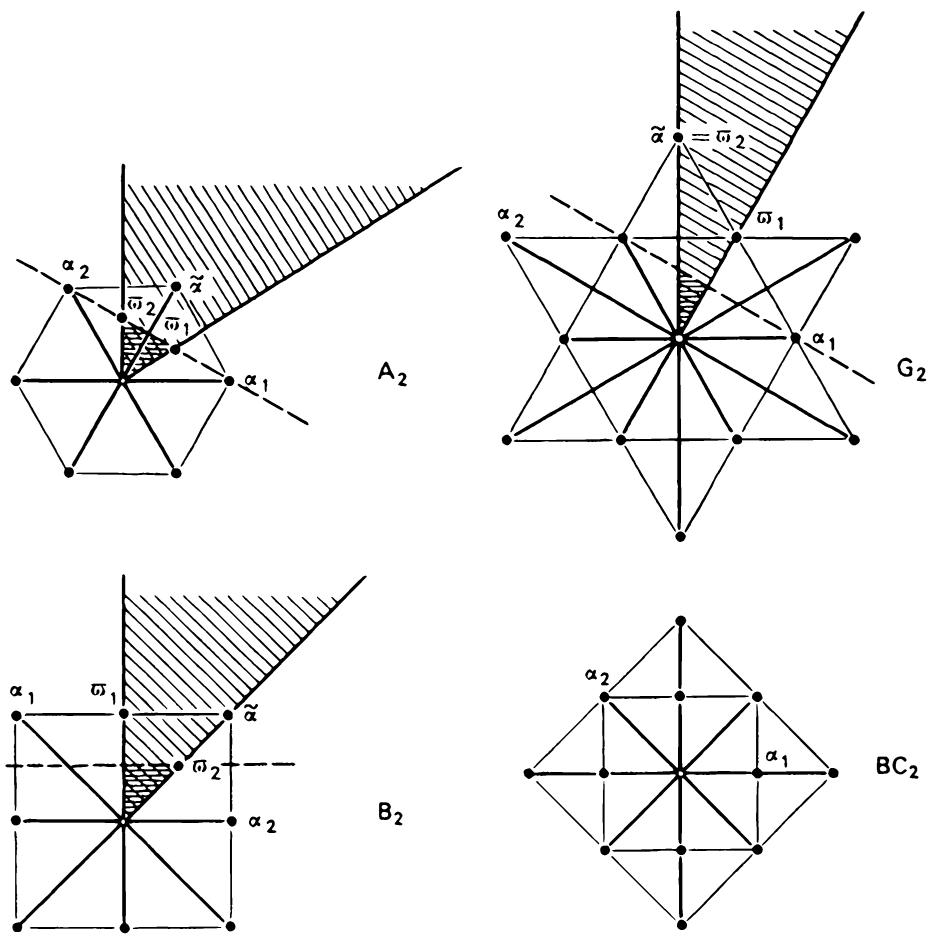
\includegraphics[keepaspectratio]{images/part002_e5dc67b9.jpg}}\\
上面的前三幅图表示 \(A_{2}\)、\(B_{2}\) 和 \(G_{2}\) 类型的根系 R。阴影区域表示与基 \((\alpha_{1},\alpha_{2})\) 相应的室 C。直线 \((x|\beta)=1\)，其中 \(\beta\) 表示

逆根系 \(R^{-}\) 的最高根；该直线以点线表示，双重阴影区域表示包含于 C 且顶点为 0 的 \(R^{-}\) 小室。

最后一幅图表示秩为 2 的唯一不可约非约化根系。
% semantic-fragments: legacy-input-seam
\relax{}
